\ifdefined\beamerclass
\else
    \def\beamerclass{beamer,aspectratio=169}
\fi
\documentclass[\beamerclass]{beamer}

\usepackage{pgfpages}
\mode<handout>{
	% \setbeamercolor{background canvas}{bg=black!20}
	\pgfpagesuselayout{2 on 1}[a4paper,border shrink=5mm]
}

\usepackage{siunitx}
\usepackage{lmodern}
\usepackage{listings}
\usepackage{amsmath}
\usepackage{bm}
\usepackage{textpos} % package for the positioning

\usepackage{pgf, tikz}
\usepackage{pgfplots}
\pgfplotsset{compat=1.13}
\usetikzlibrary{arrows, automata}


\newcommand{\dif}[1]{\ensuremath{\operatorname{d}\!{#1}}}

\usetheme{Copenhagen}
\hypersetup{pdfstartview={Fit}}
\lstset{basicstyle=\small\ttfamily,breaklines=true}

\AtBeginSection[]{
  \begin{frame}
  \vfill
  \centering
  \begin{beamercolorbox}[sep=8pt,center,shadow=true,rounded=true]{title}
    \usebeamerfont{title}\insertsectionhead\par%
  \end{beamercolorbox}
  \vfill
  \end{frame}
}

\title[Differentiable Programming]{Differentiable Programming}
\subtitle{How does pre-university calculus relate to AI and the future of computer programming?}
\author{Jonathon Hare}
\institute[]
{
  Vision, Learning and Control\\
  University of Southampton 
}
\date{}
\subject{Computer Science}
\useoutertheme{infolines}
\setbeamertemplate{headline}{} %remove headline
\setbeamertemplate{navigation symbols}{} %remove navigation symbols

\definecolor{darkblue}{RGB}{37,55,97}
\definecolor{mellowyellow}{RGB}{247,206,70}
\definecolor{almostwhite}{RGB}{254,255,255}
\definecolor{merrygreen}{RGB}{79,173,91}
\definecolor{funkyorange}{RGB}{240,154,56}

\addtobeamertemplate{footnote}{\hskip -2em}{}
\newcommand\blfootnote[1]{%
  \begingroup
  \renewcommand\thefootnote{}\footnote{#1}%
  \addtocounter{footnote}{-1}%
  \endgroup
}

\DeclareMathOperator{\softmax}{softmax}
\DeclareMathOperator{\ReLU}{ReLU}

\begin{document}

\begin{frame}[plain]
        \begin{tikzpicture}[overlay, remember picture, shift={(current page.south west)},font={\fontfamily{Montserrat-TOsF}\selectfont}]
        \fill [funkyorange,text=darkblue] (0,0) rectangle (\paperwidth, \paperheight);
        \draw (4,7) node [align=left,text=almostwhite] {\Huge \begin{tabular}{l} \textbf{Differentiate} \\ \textbf{your} \\ \textbf{Objective} \end{tabular}};
        \draw (13,1) node [align=left,text=almostwhite] {
\includegraphics[scale=0.15]{vlc.png}};
        \end{tikzpicture}
\end{frame}

\frame{
  \titlepage
}


\section{Differentiation}
\begin{frame}
\frametitle{Recap: what is the derivative of a function of one variable?}
\framesubtitle{The derivative in 1D}
\begin{columns}
\begin{column}{0.65\textwidth}
\begin{itemize}
	\setlength\itemsep{2mm}
	\item<1-> Recall that the gradient of a straight line is $\frac{\dif y}{\dif  x}$.
	\item<2-> For an arbitrary real-valued function, $f(a)$, we can approximate the derivative, $f'(a)$ using the gradient of the \emph{secant line} defined by $(a,f(a))$ and a point a small distance, $h$, away $(a+h,f(a+h))$: $f'(a) \approx \frac{f(a+h) - f(a)}{h}$.
	\begin{itemize}
		\setlength\itemsep{2mm}
		\item<3-> This expression is \textit{Newton's Quotient}.
		\item<4-> As $h$ becomes smaller, the approximated derivative becomes more accurate. 
		\item<5-> If we take the limit as $h \to 0$, then we have an exact expression for the derivative: $\frac{df}{da} = f'(a) = \lim_{h\to0} \frac{f(a+h) - f(a)}{h}$.
	\end{itemize}
\end{itemize}
\end{column}
\begin{column}{0.35\textwidth}

\begin{tikzpicture}
	\begin{axis}[
		height=6cm,
		width=6cm,
		grid=both,
		xtick distance=1,
		ytick distance=1,
		xticklabels={,,},
		yticklabels={,,},
		axis equal,
		xmin=-0.5,
		xmax=4,
		ymin=-0.5,
		ymax=4  
	]
	
	\only<1>{\addplot[color=black]{x-0.75};}
	\only<1>{\draw[color=red] (axis cs:3,2.25) -- node[right]{$\dif y$} (axis cs:3,1);}
	\only<1>{\draw[color=red] (axis cs:1.75,1) -- node[below]{$\dif x$} (axis cs:3,1);}
	\only<2-3>{\addplot[color=red]{x-0.75};}
	\only<2->{\addplot[]{0.25*x^2};}
	\only<2->{\node[pin={95:{$f(a)$}},circle,fill,inner sep=2pt,blue] at (axis cs:1,0.25) {};}
	\only<2-3>{\node[pin={110:{$f(a+h)$}},circle,fill,inner sep=2pt,blue] at (axis cs:3,2.25) {};}
	\only<4>{\addplot[color=red]{0.625*x-0.375};}
	\only<4>{\node[pin={330:{$f(a+h)$}},circle,fill,inner sep=2pt,blue] at (axis cs:1.5,0.5625) {};}
	\only<5>{\addplot[color=red]{0.525*x-0.275};}
	\only<5>{\node[pin={330:{$f(a+h)$}},circle,fill,inner sep=2pt,blue] at (axis cs:1.1,0.3025) {};}
	\end{axis}
\end{tikzpicture}

\end{column}
\end{columns}
\end{frame}

\begin{frame}
\frametitle{Recap: what are derivatives and how do we find them?}
\framesubtitle{The derivative of $y=x^2$ from first principles}
\begin{align*}
    \onslide<+->{y &= x^2 \\}
    \onslide<+->{\frac{\dif y}{\dif x} &= \lim_{h\to0} \frac{(x+h)^2 - x^2}{h} \\}
    \onslide<+->{\frac{\dif y}{\dif x} &= \lim_{h\to0} \frac{x^2 + h^2 + 2hx - x^2}{h} \\}
    \onslide<+->{\frac{\dif y}{\dif x} &= \lim_{h\to0} \frac{h^2 + 2hx}{h} \\}
    \onslide<+->{\frac{\dif y}{\dif x} &= \lim_{h\to0} (h + 2x) \\}
    \onslide<+->{\frac{\dif y}{\dif x} &= 2x}
\end{align*}
\end{frame}


\begin{frame}
\frametitle{Intuition: What does the gradient $\dif y/\dif x$ tell us}
\begin{itemize}
	\item<+-> The `rate of change' of $y$ with respect to $x$.
	\item<+-> By how much does $y$ change if I make a small change to the $x$.
\end{itemize}
\end{frame}


\begin{frame}
\frametitle{Why should we care?}
\framesubtitle{Solving a simple problem with differentiation}

\begin{columns}
\begin{column}{0.65\textwidth}
	\begin{itemize}
		\item<1-> At what angle should a javelin be thrown to maximise the distance travelled?
		\item<2-> Assume initial velocity $u=28\,\si{\meter\per\second}$ and $g=9.8\,\si{\meter\per\second\squared}$
		\item<2-> Choose to ignore launch height as it is negligable compared to distance travelled.
		\item<3-> Kinematics equations:
		\begin{align*}
			x &= u t \cos(\theta) = 28 t \cos(\theta)\\
			y &= u t \sin(\theta) - 0.5 g t^2 = 28 t \sin(\theta) - 4.9 t^2
		\end{align*}
	\end{itemize}
\end{column}
\begin{column}{0.35\textwidth}
	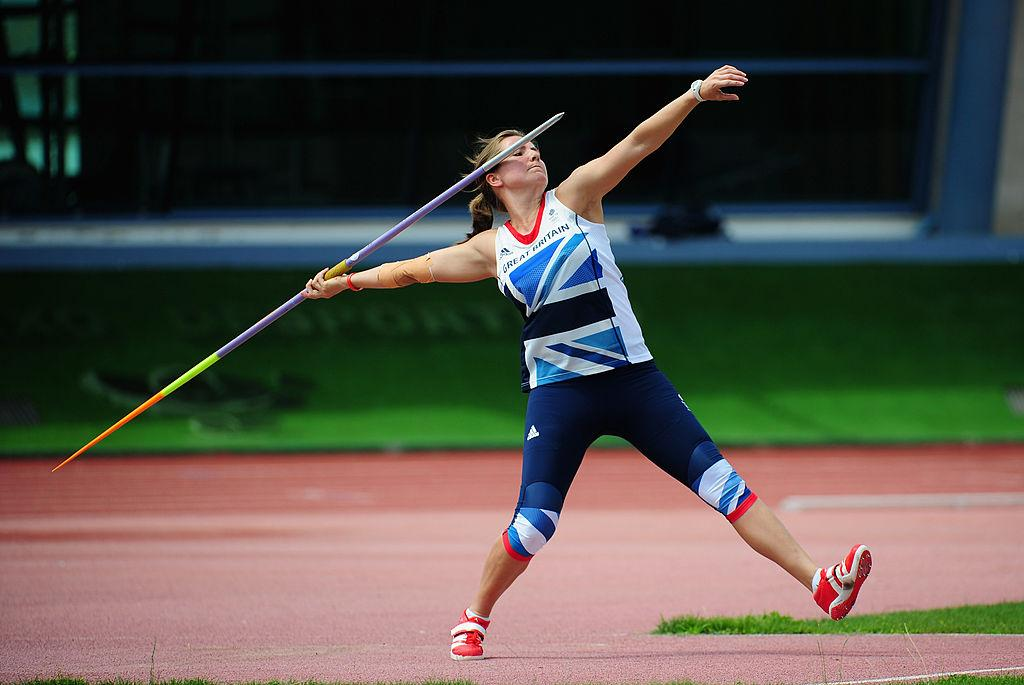
\includegraphics[width=\columnwidth]{javelin}
\end{column}
\end{columns}
\end{frame}

\begin{frame}
\frametitle{Why should we care?}
\framesubtitle{Solving a simple problem with differentiation}

\begin{columns}
\begin{column}{0.65\textwidth}
	\vspace{-1ex}
	\begin{align*}
		x &= 28 t \cos(\theta)\\
		y &= 28 t \sin(\theta) - 4.9 t^2
	\end{align*}\vspace{-3ex}
	\begin{itemize}
		\item Javelin hits ground when $y = 0$ and we only care about $t>0$:
		\begin{align*}
		0 &= 28 t \sin(\theta) - 4.9 t^2 \\
		%4.9 t^2 &= 28 t \sin(\theta) \\
		%4.9 t &= 28 \sin(\theta) \\
		\implies t &= \frac{28}{4.9} \sin(\theta)
		\end{align*}
		\item Substituting into the horizontal component: \begin{align*}
		x &= 28 \frac{28}{4.9} \sin(\theta) \cos(\theta) = 80 \sin(2\theta)
		\end{align*}
	\end{itemize}
\end{column}
\begin{column}{0.35\textwidth}
	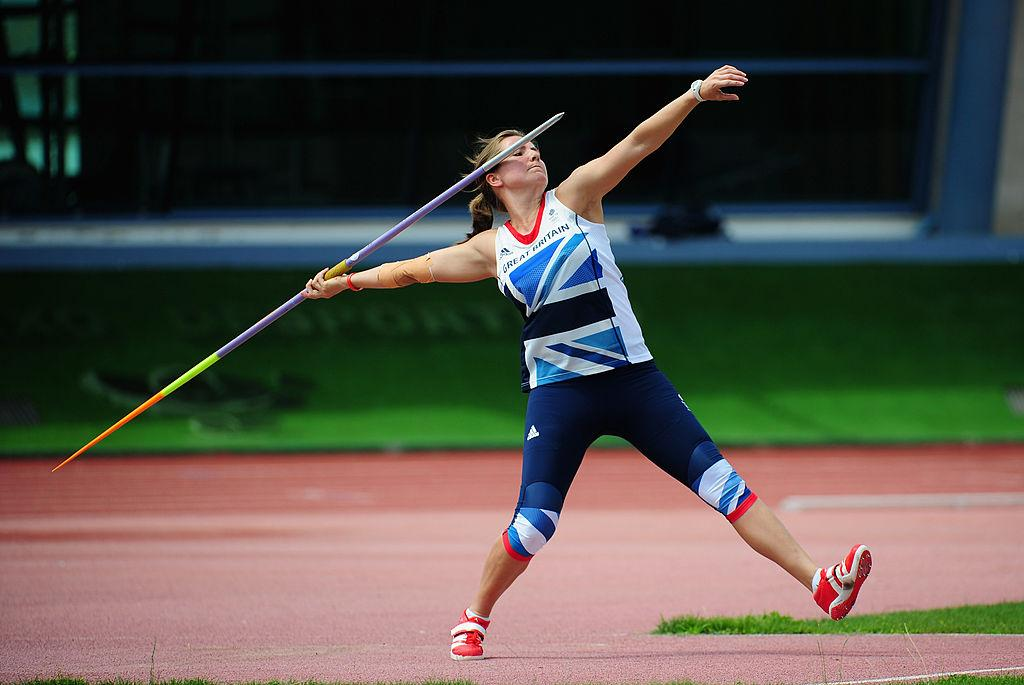
\includegraphics[width=\columnwidth]{javelin}
\end{column}
\end{columns}
\end{frame}


\begin{frame}
\frametitle{Why should we care?}
\framesubtitle{Solving a simple problem with differentiation}

\begin{columns}
\begin{column}{0.65\textwidth}
	\begin{equation*}
	\begin{aligned}
    \max_{\theta} \quad & 80 \sin(2\theta)\\
    \textrm{s.t.} \quad & 0 \leq \theta \leq \frac{\pi}{2}
    \end{aligned}
    \end{equation*}

    \uncover<2->{
    Compute derivative w.r.t $\theta$ and set to zero:
    \begin{align*}
    	0 &= \frac{\dif (80 \sin(2\theta))}{\dif \theta}\\
    	  &= 160 \cos(2\theta)\\
    	  \implies \theta &= \frac{1}{2}\cos^{-1}(0) = \frac{\pi}{4}
    \end{align*}
    }
	
	\uncover<3->{
		\textbf{Irrespective of the initial velocity maximum distance is acheived at $45\si{\degree}$}.
	}
\end{column}
\begin{column}{0.35\textwidth}
	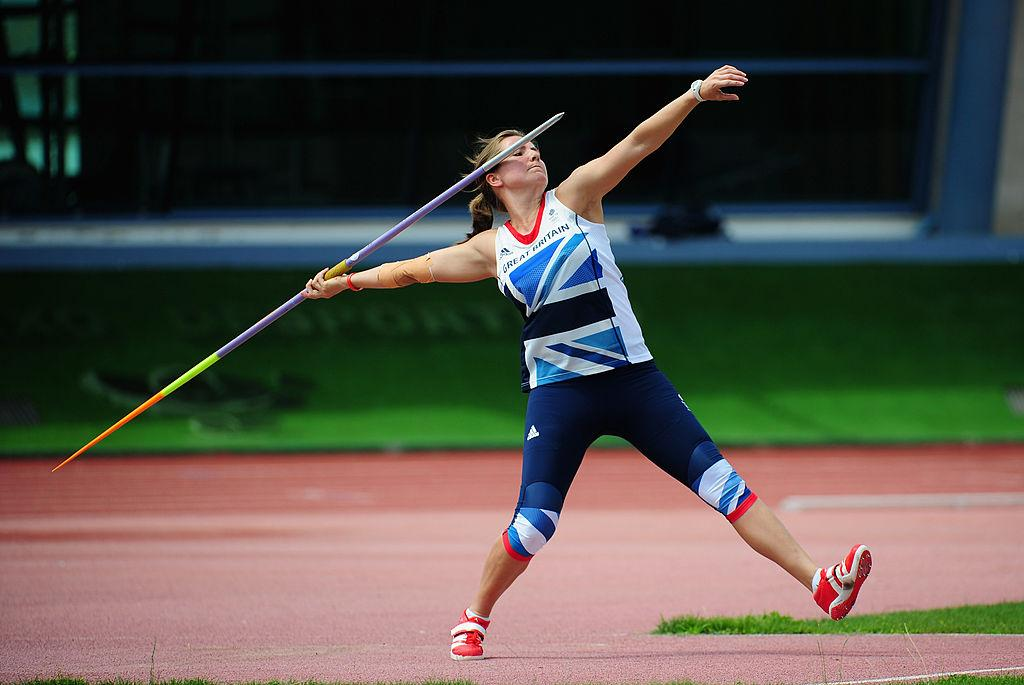
\includegraphics[width=\columnwidth]{javelin}
\end{column}
\end{columns}
\end{frame}


\begin{frame}
\frametitle{Abstraction: Solving problems by minimising an objective}

\begin{itemize}
	\item<+-> To compute the parameter (angle) for the javelin example we \emph{maximised} the equation for distance travelled.
	\item<+-> We can solve all kinds of problems if we can:
	\begin{itemize}
	 	\item \textbf{formulate} a \emph{loss} or \emph{cost} function.
	 	\item<+-> \textbf{minimise} the loss with respect to the parameter(s)\footnote{Note: maximising a distance is the same as minimising a negative distance}.
	 \end{itemize} 
	 \item<+-> Problems:
	 \begin{itemize}
	 	\item The loss must be differentiable (or rather you must be able to compute or estimate its gradient somehow).
	 	\item Some loss functions might have many minima; you might have to settle for finding a sub-optimal one (or a saddle-point).
	 	\item The loss function could be arbitrarily complex... you might not be able to analytically compute the solution (or the gradient).
	 \end{itemize}
\end{itemize}

\end{frame}

\begin{frame}
\frametitle{A simple algorithm for minimising a function}
\framesubtitle{Gradient Decent}

\begin{columns}
\begin{column}{0.65\textwidth}

\begin{itemize}
	\item<+-> How can you numerically estimate the value of the parameter $\theta$ that minimises a loss function, $\ell(\theta)$?
	\item<+-> Really intuitive idea: starting from an initial guess, $\theta_0$, take small steps in the direction of the negative gradient.
\end{itemize}

\uncover<+->{
\center
Gradient Descent: \\[0.7em]
$\theta_{i+1} = \theta_{i} - \gamma \frac{\dif \ell}{\dif \theta}$
where $\gamma$ is the \emph{learning rate}

}


\end{column}
\begin{column}{0.35\textwidth}

\begin{tikzpicture}
	\begin{axis}[
		height=6cm,
		width=6cm,
		grid=both,
		xtick distance=1,
		ytick distance=1,
		xticklabels={,,},
		yticklabels={,,},
		axis equal,
		xmin=-3,
		xmax=4 
	]
	
	\only<1->{\addplot[]{0.25*x^2};}
	\only<2->{\node[pin={150:$\theta_0$},circle,fill,inner sep=2pt,blue] at (axis cs:3,2.25) {};}
	\only<3->{\node[pin={150:$\theta_1$},circle,fill,inner sep=2pt,blue] at (axis cs:2,1) {};}
	\only<3->{\node[pin={150:$\theta_2$},circle,fill,inner sep=2pt,blue] at (axis cs:1,0.25) {};}
	
	\end{axis}
\end{tikzpicture}

\end{column}
\end{columns}

\end{frame}

\begin{frame}
\frametitle{Javelin throwing again, but with Python code}

\end{frame}


\begin{frame}
\frametitle{Derivatives of more general functions}

\begin{itemize}
	\item<1-> Almost all complex functions can be broken into simpler parts (often with very simple derivatives).
	\item<1-> You can add (or subtract) sub-functions, multiply (or divide) sub-functions and make functions of functions.
	\begin{itemize}
		\item The sum rule, product rule and chain rule tell you how to differentiate these.
	\end{itemize}
	\item<2-> If you break down functions into their constituent parts computing the derivative becomes very easy
	\item<2-> Example: the $\sin$ function can be written in terms of exponentials (Euler's formula) and the derivative of an exponential $e^x$ is just $e^x$\dots
\end{itemize}
\end{frame}

\begin{frame}
\frametitle{Derivatives of more general functions}

\begin{itemize}
	\item<1-> Most interesting functions that we might want to work with have more than one parameter that we might want to optimise.
	\begin{itemize}
		\item<1-> In many real applications it can be \emph{millions} of parameters.
	\end{itemize}
	\item<2-> Partial derivatives $\frac{\partial f}{\partial x_i}$ let us compute the gradient of the $i$-th parameter by holding the other parameters constant.
	% \item<3-> In general, the partial derivative of a function $f(x_1,\dots,x_n)$ at a point $(a_1,\dots,a_n)$ is given by: $\frac{\partial f}{\partial x_i}(a_1,\dots,a_n) = \lim_{h\to0}\frac{f(a_1\dots,a_i+h,\dots,a_n)-f(a_1\dots,a_i,\dots,a_n)}{h}$.
\end{itemize}
\end{frame}

\section{Back to programming}

\begin{frame}
\frametitle{Programming is really just function composition and control statements}

\begin{itemize}
	\item<+-> At the end of the day computer programs are just compositions of really simple functions that computer processors can compute: arithmetic operations (add, multiply, divide, ...), logical operations (and, or, not, comparisons...), operations that move data, etc.
	\item<+-> Many of these primitive operations have \emph{well defined} gradients with respect to their operands.
	\item<+-> The chain rule tells us how to compute gradients of composite functions.
\end{itemize}

\begin{block}<+->{}
So, in principle we can find the optimal ``parameters'' of a computer program designed to solve a specific task by following the gradients to optimise it.
\end{block}

    
\end{frame}

\begin{frame}[fragile]
\frametitle{Differentiating Branches}

\begin{columns}
	\column{.45\textwidth}
    \begin{block}<1->{Code - \emph{if-else} statement}
    \begin{minipage}[c][2.5cm][c]{\linewidth}\begin{lstlisting}[language=python]
if a > 0.5:
    b = 0
else:
    b = 2 * a
\end{lstlisting}
	\end{minipage}
    \end{block}

\column{.45\textwidth}
	\begin{block}<1->{Math}
	\begin{minipage}[c][2.5cm][c]{\linewidth}\vspace{-0.5cm}%
	\begin{align*}
	b(a) &= \begin{cases} 0 & \text{if } a > 0.5 \\ 2 a & \text{if } a \leq 0.5 \end{cases} \\ 
	\frac{\partial b}{\partial a} &= \begin{cases} 0 & \text{if } a > 0.5 \\ 2 & \text{if } a \leq 0.5 \end{cases} 
	\end{align*}
   \end{minipage}
	\end{block}
\end{columns}
\end{frame}

\begin{frame}[fragile]
\frametitle{Differentiating Loops}
\begin{columns}
	\column{.45\textwidth}
    \begin{block}<1->{Code - \emph{for loop} statement}
    \begin{minipage}[c][3.5cm][c]{\linewidth} 
\begin{lstlisting}[language=python]
b = 1
for i in range(3):
    b = b + b * a
\end{lstlisting}
	\end{minipage}
    \end{block}

\column{.45\textwidth}
	\begin{block}<1->{Math}
	\begin{minipage}[c][3.5cm][c]{\linewidth}\vspace{-0.75cm}%
	\begin{align*}
	b_0 &= 1 \\
	b_1 &= b_0 + b_0 a = 1 + a \\
	b_2 &= b_1 + b_1 a = 1 + 2a + a^2 \\
	b_3 &= b_2 + b_2 a = 1 + 3a + 3a^2 + a^3 \\
	\frac{\partial b}{\partial a} &= 3 + 6a + 3a^2
	\end{align*}
   \end{minipage}
	\end{block}
\end{columns}
\end{frame}



\begin{frame}
\frametitle{Can all programs be differentiable?}

\begin{itemize}
	\item<+-> We can differentiate through lots of types of programs and algorithms (even the Gradient Decent algorithm is itself differentiable!), but...
	\item<+-> not every operation or function has \emph{useful} gradients
	\begin{itemize}
		\item<+-> discontinuities, large areas of zero-gradient, ...
	\end{itemize}
	\item<+-> Computer science researchers are actively developing mathematical `tricks' to circumvent many of these problems.
	\begin{itemize}
		\item \emph{Relaxations} of functions that behave almost the same, but have well defined gradients.
		\item \emph{Reparameterisations} of functions involving randomness.
		\item \emph{Approximations} of useable gradients for functions that have ill-posed gradients.
	\end{itemize}
\end{itemize}
\end{frame}


% \begin{frame}
% \frametitle{Do I really have to do the differentiation manually?}

% \begin{itemize}
% 	\item There are three ways to perform differentiation:
% 	\begin{itemize}
% 		\item<+-> analytically;
% 		\item<+-> numerically;
% 		\item<+-> automatically.
% 	\end{itemize}
% \end{itemize}

% \begin{block}<+->{}
% Automatic Differentiation is key to differentiating programs with millions of parameters, but as the `programmer' \textbf{you} still need to have a really good intuition and understanding of what the implications of composing many functions will be on the gradients of the parameters with respect to the loss for optimisation to work successfully.
% \end{block}

% \end{frame}

\begin{frame}
\frametitle{What kinds of functional building blocks are common?}

\begin{itemize}
	\item<+-> Today, the most common operations with parameters are:
		\begin{itemize}
			\item \emph{Vector addition}: the input vector to a function is added to a vector of weights.
			\item \emph{Vector-Matrix multiplication}: the input vector to the function is multiplied with a matrix of weights.
			\item \emph{Convolution}: the input vector (or matrix...) is `convolved' with a set of weights.
			\item (in all these cases `weights' are the parameters which are learned)
		\end{itemize}
	\item<+-> The above operations are \emph{linear}, so they are often combined with element-wise nonlinearities; e.g.:
	\begin{itemize}
		\item $\max(0, x)$ aka $\ReLU$.
		\item $\tanh(x)$.
		\item $\frac{1}{1+e^{-x}}$ aka \emph{sigmoid} or the \emph{logistic} function. 
	\end{itemize}
\end{itemize}
\end{frame}


\section{Real Examples of Differentiable Programming}

\begin{frame}
\frametitle{Playing Games}

\begin{itemize}
	\item You can use differentiable programming to write (and train) `agents' that can play games.
	\item It can be hard to get a gradient from a single game involving many moves, but there is a clever trick which allows good estimates of gradients to be created over the average of \emph{many} games.
	\item This is broadly the area of what is called \emph{reinforcement learning}.
\end{itemize}

\begin{center}
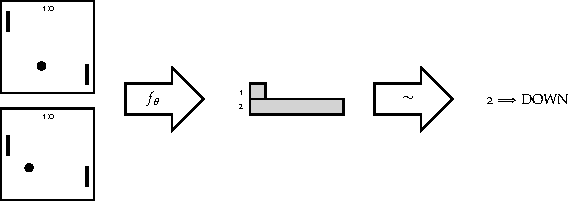
\includegraphics[width=0.75\textwidth]{pong}
\end{center}
\end{frame}

\begin{frame}
\frametitle{Playing Games}
\framesubtitle{Demo: AlphaStar}
\end{frame}

\begin{frame}
\frametitle{Object detection}

\begin{itemize}
	\item Consider a function that takes an image as input and produces an array of \emph{bounding boxes} and corresponding \emph{labels}.
	\item With enough \emph{training data} we can learn the parameters required to detect objects in images.
\end{itemize}

\begin{center}
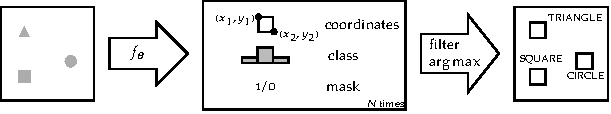
\includegraphics[width=0.75\textwidth]{objdet-sets}
\end{center}
\end{frame}

\begin{frame}
\frametitle{Object detection}
\framesubtitle{Demo}

\end{frame}

% \begin{frame}
% \frametitle{Face detection and recognition}

% \begin{itemize}
% 	\item Consider a function that takes an image as input and produces an array of \emph{bounding boxes}.
% 	\item With enough \emph{training data} we can learn the parameters required to detect faces in images.
% 	\item With some clever training tricks (in the loss function) we can also make the function return a feature for each box that describes the content, such that pictures of the same person have very similar features.
% \end{itemize}

% \end{frame}

% \begin{frame}
% \frametitle{Face detection and recognition}
% \framesubtitle{Demo}
% \end{frame}


\begin{frame}
\frametitle{Drawing}

\begin{itemize}
	\item We could envisage a differentiable function that takes in a set of line coordinates and turns them into an image...
	\item With such a function we can optimise the line coordinates so they e.g. match a photograph, thus automatically creating a \emph{sketch}.
\end{itemize}
\end{frame}

\begin{frame}
\frametitle{Drawing}
\framesubtitle{Demo}

\center
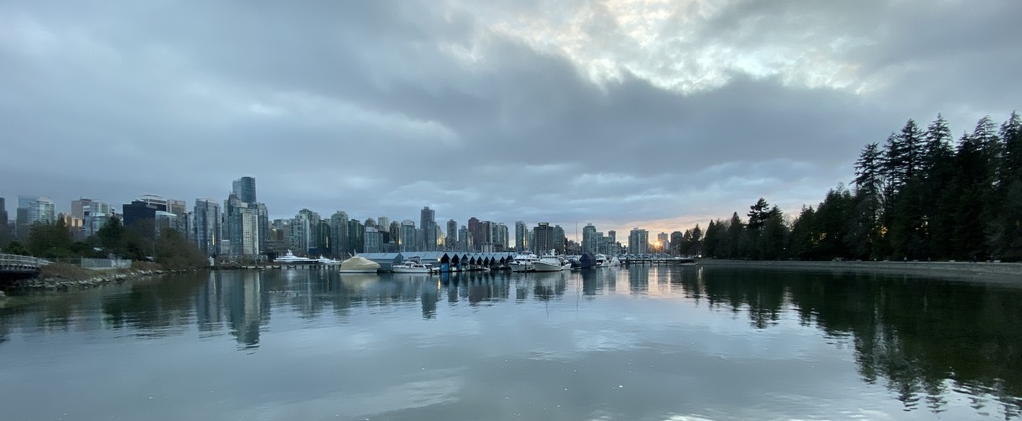
\includegraphics[width=\textwidth]{vancouver.jpg}

\end{frame}

\begin{frame}
\frametitle{Drawing}
\framesubtitle{Demo}

\end{frame}

\section{Where is this all going?}

\begin{frame}
\frametitle{Software 2.0}
\framesubtitle{There is a revolution happening and you're going to be part of it}

\centering
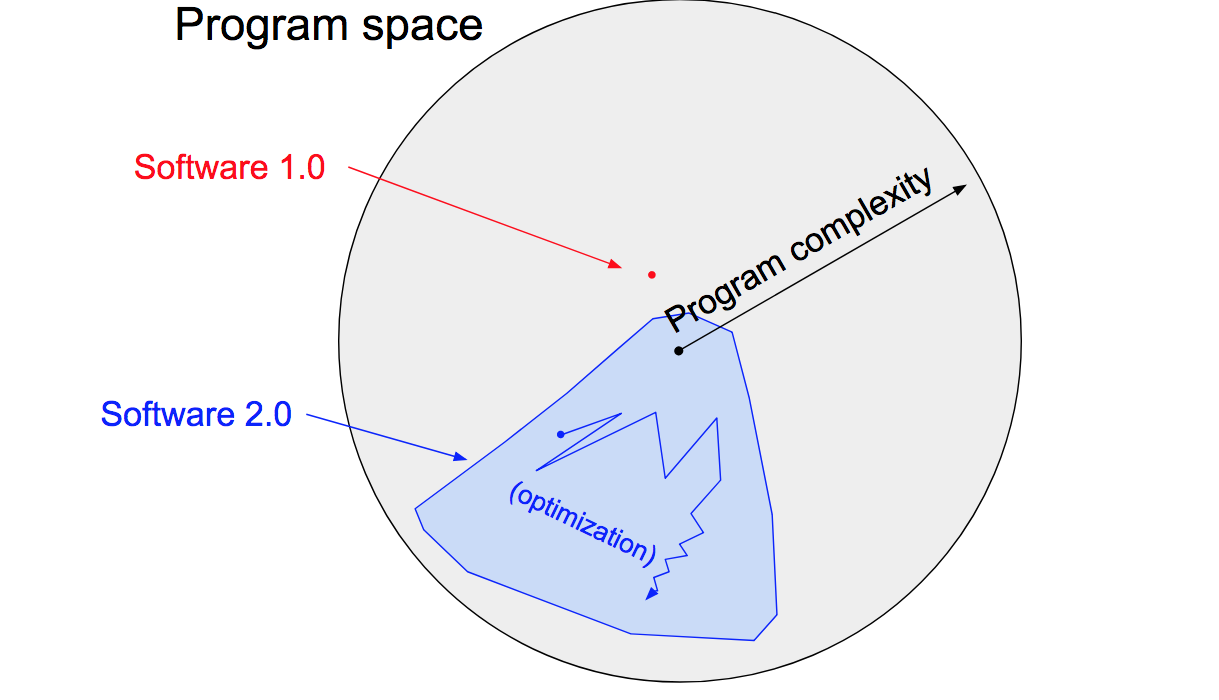
\includegraphics[scale=0.24]{software2_0}\\
Image credit: Andrei Karpathy \url{https://karpathy.medium.com/software-2-0-a64152b37c35}
\end{frame}

\section{Any Questions?}

\end{document}